\documentclass[12pt]{article}

\usepackage{sbc-template}

\usepackage{listings} %code
\usepackage{syntax} %grammar
\usepackage{graphicx,url} %figures
\usepackage{lscape}

\usepackage[utf8]{inputenc}
\usepackage[T1]{fontenc}
% UTF-8 encoding is recommended by ShareLaTex

\usepackage{algorithm2e}

\sloppy

\title{Anotações sobre Deep Neuroevolution}

\author{Ricardo Henrique Remes de Lima \inst{1}}

\address{Departamento de Informática\\
	Universidade Federal do Paraná (UFPR)\\
  \email{ricardo.hrlima@gmail.com}
}

\begin{document} 

\maketitle

\section{Convolutional Neural Networks}

\section{Deep Neuroevolution}

\section{Approach}

This section will present the details about the proposed approach, describing the tools used, the design of the grammar, how the mapping process creates the CNNs and how the search engine works to improve the solutions.

\subsection{Tools}

Here we present the tools that were used in order to better understand the decisions made in further steps of the approach. The technologies used are listed below:

\begin{itemize}
	\item \textbf{Python v3.6}: The use of the Python\footnote{https://www.python.org} language is supported by the well known frameworks that are used in machine learning projects, as well as offering a simple syntax to improve productivity. 
	
	\item \textbf{Tensorflow}: The Tensorflow\footnote{https://www.tensorflow.org} framework is a powerful open-source library for high performance numerical computation. Its flexible architecture allows easy deployment of computation across a variety of platforms.
	
	\item \textbf{Keras}: A Python Deep Learning library. Keras \footnote{https://keras.io/} is a high-level neural networks API, written in Python and capable of running on top of Tensorflow, CNTK\footnote{https://github.com/Microsoft/cntk} or Theano\footnote{https://github.com/Theano/Theano}. Designed to enable fast experimentation.
\end{itemize}


\subsection{Grammar}


The GE Grammar has the task of defining a generic structure that allows the creation of different variations of a program according to the problem. The rules and productions are usually used to describe ``blocks'' of routines and parameters that the program has, and also how these blocks connect to each other.


To design the CNNs we selected some of the most common layers implemented in the Keras framework, as well as some of the available parameters that comes with them. The options are listed below:


\begin{itemize}
	\item Convolution Layer: Filters, Kernel size, Activation function
	
	\item Max/ Average Pooling: Pooling size, Padding
	
	\item Dense: Units, Activation function
	
	\item Dropout: Drop rate
	
	\item Filters: 32, 64
	
	\item Kernel size: (3, 3), (5, 5)
	
	\item Activation function: Relu, Tahnm, Linear
	
	\item Pooling size: (2, 2), (4, 4)
	
	\item Padding: Valid, Same
	
	\item Number of Units: 32, 64
	
	\item Drop rate: rand[0, 1]
\end{itemize}


A first version of a grammar using the CNN components can be seen in Figure \ref{fig:cnn-grammar}. The rules and productions were designed to ensure the creation of valid CNN models, as well as giving the opportunity to grow in size and complexity.


\begin{figure}[!htb]
	\begin{grammar}
		<cnn> ::= <conv> <c\_layer> <d\_layer> <dense>
		
		<c\_layer> ::= <c\_layer> <c\_layer> | <c\_node> | '\&'
		
		<d\_layer> ::= <d\_node> <d\_node> | <d\_node> | '\&'
		
		<c\_node> ::= <conv> | <maxpool> | <avgpool>
		
		<d\_node> ::= <dense> | <dropout>
		
		<conv> ::= `Conv2D' <filters> <k\_size> <activation>
		
		<dense> ::= `Dense' <units>
		
		<dropout> ::= `Dropout' <rate>
		
		<maxpool> ::= `MaxPooling2D' <p\_size> <padding>
		
		<avgpool> ::= `AveragePooling2D' <p\_size> <padding>
		
		<activation> ::= `relu' | `tanh' | `linear'
		
		<padding> ::= `valid' | `same'
		
		<filters> ::= `32' | `64'
		
		<k\_size> ::= `(3, 3)' | `(5, 5)'
		
		<p\_size> ::= `(2, 2)' | `(4, 4)'
		
		<units> ::= `32' | `64'
		
		<rate> ::= `[0.0, 1.0]'
		
	\end{grammar}
	\caption{Proposed grammar to generate CNNs.}
	\label{fig:cnn-grammar}
\end{figure}


\subsection{Mapping}


The mapping is responsible to translate the genotype of a solution into the correspondent phenotype through the grammar. Generating CNNs with this approach is very simple, because we just have to define which layers will be used, in which sequence and also define the values of the parameters of each of these layers.


The proposed grammar was designed to allow the creation of both a small CNN with just one \textit{convolution} layer and one \textit{dense} layer, as well as CNNs as big as we want, using many \textit{convolution}, \textit{pooling}, \textit{dense} and \textit{dropout} layers. Because of this flexibility in generating the CNNs, some rules were defined to ensure that most valid models would be created considering how Keras works. The rules are as follows:


\begin{enumerate}
	\item All models start with a \textit{convolution} layer
	
	\item All models end with a \textit{dense} layer
	
	\item The last layer must have the output shape as a 1D array and length as the number of classes
	
	\item The last layer must have the activation function set to \textit{softmax}
	
	\item The first \textit{dense} layer is preceded by a \textit{fatten} layer
\end{enumerate}


Even with these rules, invalid models are still possible, in those cases we can apply a poor fitness to the solution, so it will be replaced during the search. Figure \ref{fig:cnn-map-scheme} illustrates how a CNN is built by connecting the layers, noting that fully connected layers (\textit{dense}, \textit{dropout}, etc) will only be available to be added after at least one \textit{convolution} is added to the architecture, and after that, no more \textit{convolution} layer can be added.


\begin{figure}[!htb]
	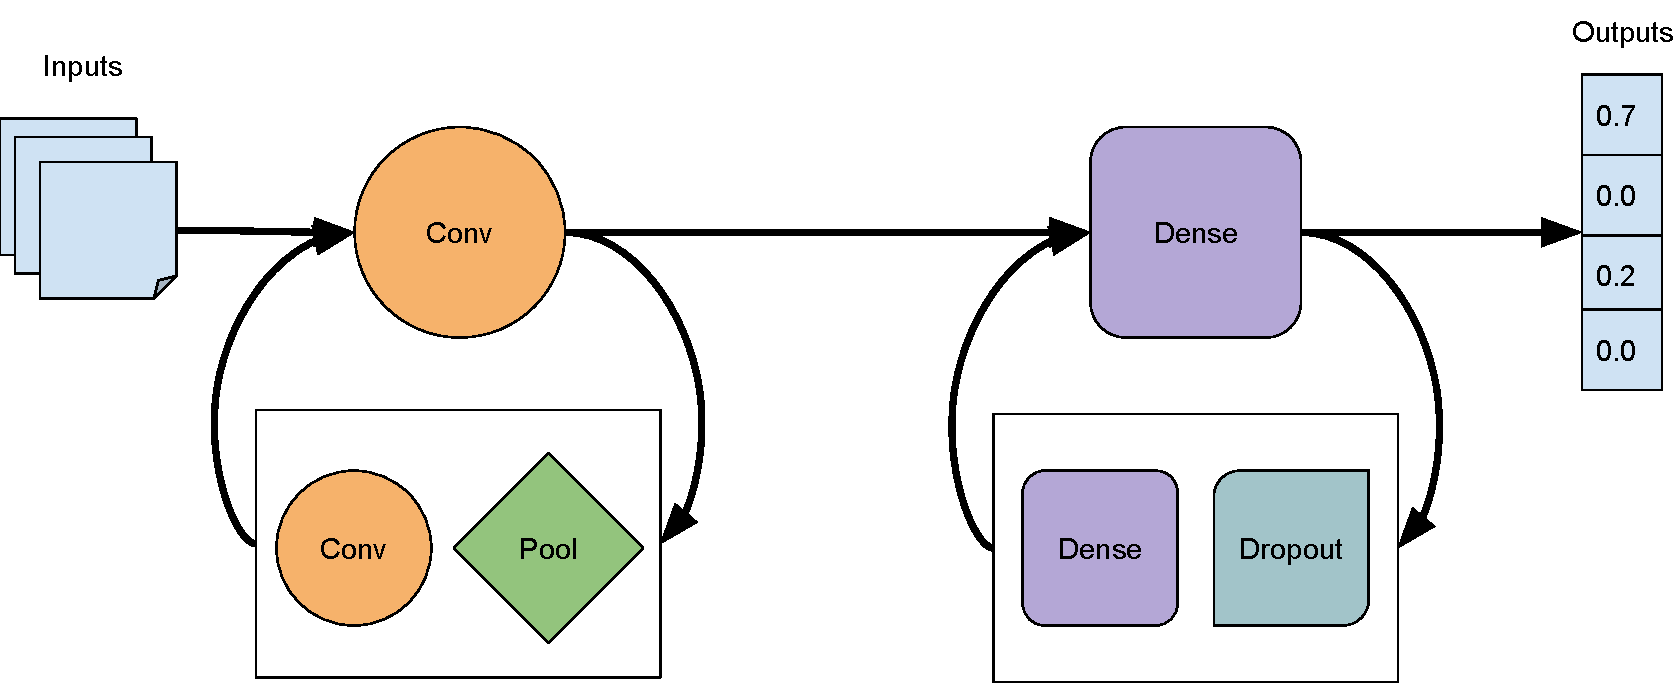
\includegraphics[width=\linewidth]{images/mapping-example.pdf}
	\caption{Example of mapping expansion of a CNN model.}
	\label{fig:cnn-map-scheme}
\end{figure}


The way Keras can be used to build CNN models is very simple. We can create a \textit{Sequential} model, that is a linear stack of layers, and add the desired components. Figure \ref{fig:cnn-model} shows an example of a simple CNN. It is also possible to save a model to a \textit{json} format, as well as load a model, but not the weights, from a \textit{json} file.


\begin{figure}[!htb]
	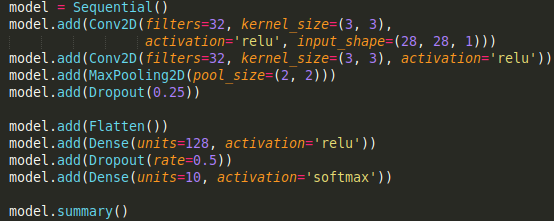
\includegraphics[width=\linewidth]{images/cnn-model-example.png}
	\caption{Simple CNN using Python and Keras.}
	\label{fig:cnn-model}
\end{figure}


\begin{figure}
	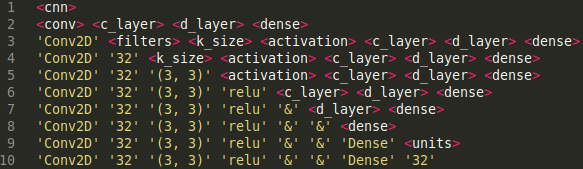
\includegraphics[]{images/expansion_example.png}
\end{figure}


\subsection{Search}

\bibliographystyle{plain}
\bibliography{referencias}

\end{document}